\documentclass{IEEEtran}
%% BIbliography Setup - Biblatex please
\usepackage[
backend=biber,
style=ieee,
]{biblatex}
\addbibresource{DBT_References.bib}

%% Packages
\usepackage{caption}
\usepackage [none] {hyphenat} 
\usepackage{siunitx}
\usepackage{graphicx}
\usepackage{amsmath}
\usepackage{subcaption}
\usepackage{pdfpages}
\usepackage{booktabs}
\usepackage{svg}

%% Packages added by Jan
\usepackage[colorlinks=true,linkcolor=black,anchorcolor=black,citecolor=black,filecolor=black,menucolor=black,runcolor=black,urlcolor=black]{hyperref}
\usepackage[nameinlink,capitalise]{cleveref}
\usepackage{makecell}

\markboth{Centre for Doctoral Training in Composites Science, Engineering and Manufacturing - Design, Build and Test, CDT 22}{Last Name \MakeLowercase{\textit{et al.}}: Title}

\title{CDT 22 - Design, Build and Test.\\ Sequential Instabilities for Actuating Aerodynamic Surfaces}
\author{A. Biqai$^1$, R.M. Birgisson$^1$, J. Lavazza$^1$, M. Leeder$^1$, M. Lillywhite$^1$, W. Mahoney$^1$, J. Rifai$^1$, G. Sancak$^1$, J. M. Uszko$^1$ and A. Williams$^1$\\
	$^1$Bristol Composites Institute, University of Bristol, Queens Building, Bristol, BS8 1TR, United Kingdom\\
	\textit{$^1$qz22653@bristol.ac.uk, $^1$qh18199@bristol.ac.uk, $^1$jacopo.lavazza@bristol.ac.uk, $^1$matthew.leeder@bristol.ac.uk, $^1$yn21907@bristol.ac.uk, $^1$will.mahoney@bristol.ac.uk, $^1$joe.rifai@bristol.ac.uk, $^1$gokhan.sancak@bristol.ac.uk, $^1$jm.uszko@bristol.ac.uk, $^1$go22666@bristol.ac.uk}}
\begin{document}
	\maketitle
	
	\begin{abstract}
        Structural instability is traditionally seen as a failure mode to be avoided. However, in recent years multiple novel designs which exploit the rapid, large scale deformations seen in nonlinear structures have been developed. A development of this design approach is the investigation of using interacting instabilities, a well known and studied phenomena, for useful functionality in deployment of morphing structures. In this work we seek to demonstrate the feasibility of the exploitation of interacting, sequential instability to achieve functionality for a wing mounted control surface for the application of gust load alleviation. This builds on a novel concept for a passively actuated spoiler first proposed by Wheatcroft et al. in \cite{Wheatcroft_2023}. To display feasibility, a bespoke experimental setup was designed to initiate sequential instability between a clamped-clamped Euler strut and a composite laminate shaped to the profile of a NACA 3412 aerofoil. Results from experimentation imply that a sequential instability was successful in achieving rapid deployment. The results are compared to models of the test setup produced in Abaqus, to assure validity of the experiment and models produced. The captured data also provides insight into the behaviour of a deployment system that exploits sequential instability which should be of use for further development of the presented concept.
	\end{abstract}
	
	\section{Introduction}
		\subsection{Control Surfaces for Gust Load Alleviation}
		Gust loads are well known as a source of potential catastrophic failure in aircraft structures; with rare, extreme gusts in particular being a source of the maximum loads that an aircraft may experience. \cite{Wu2019,Guo_2015}. Aircraft structural requirements are driven by extreme cases to prevent failure, despite operating in far less intense loading environments for the majority of the aircraft's service life \cite{Li2021}. The added capability to cope with extreme gust loads is unnecessary most of the time and comes with an associated parasitic mass increase, which causes reduced fuel efficiency of the aircraft. 
		
		Gust load alleviation (GLA) systems aim to reduce the effect of gust loads while minimising mass increase by altering the aerodynamic profile of the wing \cite{Li_2022}. Active control surfaces such as ailerons, spoilers have been used to achieve this \cite{Li_2022}. However, such control surfaces utilise conventional, active actuation mechanisms such as hydraulic or electro-mechanical actuators \cite{QI_2011}. These mechanisms still introduce significant mass and complexity to aircraft which still results in a decrease to fuel efficiency and an increase in cost and manufacture time. A passively actuated GLA system is a mechanism which is able to deploy using the deformation of the wing itself. These are attractive as they are typically simpler and require no external energy \cite{Li_2022}. A lightweight, passive GLA system could provide the necessary gust alleviation whilst keeping the parasitic mass added to the aircraft low.  
		
		\subsection{Sequential Instabilities}
		A potential actuation mechanism for a passive GLA system is through the utilisation of structural instabilities. The traditional view on structural instability, known as '\textit{Buckliphobia}', is largely negative and the presence of buckling is seen as a failure mode. '\textit{Buckliphillia}' is an emerging design philosophy which seeks to exploit instability as a design feature \cite{Reis_2015}. By deliberately designing a structure to become unstable in predictable ways, useful functionality can be achieved, such as large and rapid deflections in shape morphing structures. This approach has potential application for aircraft design as the deflections necessary for actuating a control surface could be achieved through a '\textit{Buckliphillic}' approach. Examples of structural instability exploited for functionality in control surface actuation include: A bistable composite trailing edge flap \cite{Daynes2010} and a non-linear spring wing-tip device for gust load alleviation \cite{Castrichini2017}.
		
         By extending this approach to include the exploitation of interacting instabilities, new interesting and novel designs for dynamic structures can be produced. Buckling modes are able to interact with each other and interacting instabilities occur when two or more buckling modes share coincident critical points \cite{Wheatcroft_2023}. Whilst the adoption of structural instability as a design feature has received much attention in recent years and shifted the view of instability to be more positive, interacting instabilities are still viewed primarily as a failure mechanism. A novel concept for a passively-actuated spoiler proposed by Wheatcroft et al. exploits sequential, interacting instabilities to produce a large post buckling deflection in a bistable, constant curvature, composite laminate \cite{Wheatcroft_2023}. A pair of instabilities can be considered sequential when an instability in one system triggers a subsequent instability in another. Utilising sequential instability as a design feature enables refined control over the device deployment, whilst eliminating the need for heavy, active deployment mechanisms.
		
		\subsection{Pop-up Spoiler Concept}
		\begin{figure}[!h]
            \captionsetup{justification=centering}
			\centering{}
			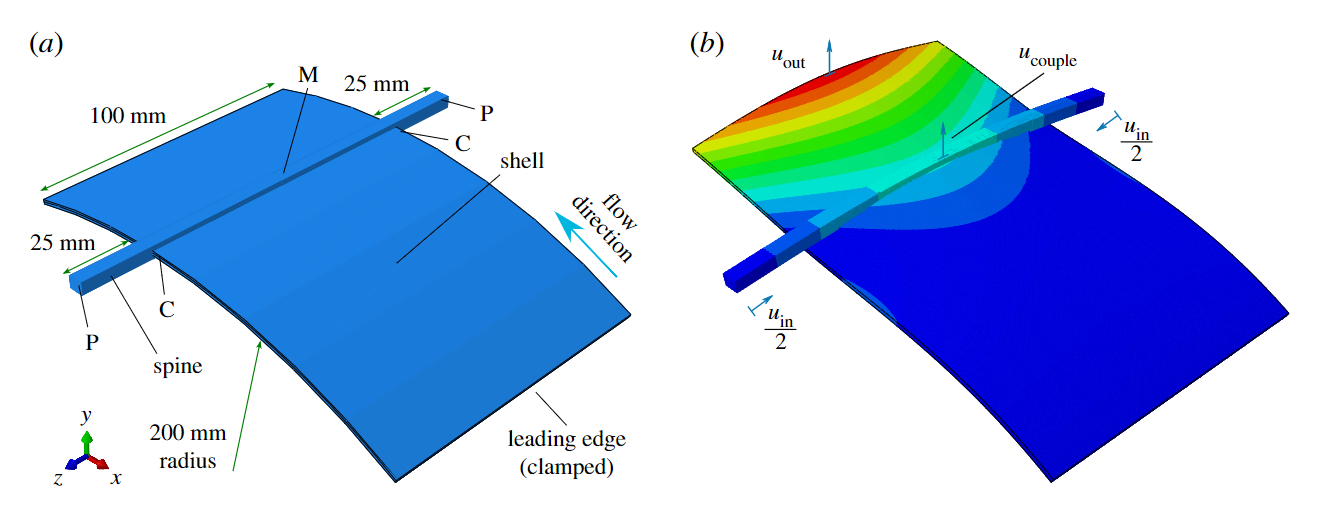
\includegraphics[width=0.5\textwidth]{IntroductionImages/Concept.png}
            \caption{FE model of original concept for passively actuated pop-up spoiler, \textbf{(a)}: undeployed state, \textbf{(b)} deployed state. \\ (Taken from \cite{Wheatcroft_2023})}
			\label{fig:OGConcept}
		\end{figure}
	
		The original novel spoiler concept proposed by Wheatcroft et al. is shown in \cref{fig:OGConcept} and is constituted from an Euler strut and a bistable composite laminate. In the original work the laminate is a constant curvature. For this investigation, the concept is extended to include a composite laminate shaped to the upper surface of an aerofoil to better resemble the application for a wing mounted spoiler. It is envisioned that strain caused by deflection in a wing under heavy load will cause the strut to buckle into a mode that subsequently causes the laminate to buckle, creating a sequential instability. A representative bar and spring diagram for this system is shown in \cref{fig:BarNSpring}. From this diagram the deployment mechanism which exploits the  interaction between the a pair of instabilities can clearly be seen. This should produce the ideal behaviour, shown in \cref{fig:DesiredPath}, where the deflection of the laminate, $u_{out}$, is plotted as a function of the enforced axial compressive deformation of the Euler strut, $u_{in}$. Initially $u_{out}$ grows slowly as $u_{in}$ increases. Once $u_{in}$  reaches a critical value, it results in the system traversing an unstable region, resulting in a dynamic deflection and a large, rapid increase to $u_{out}$.

		\begin{figure}[!h]
			\centering
			\includesvg[width=0.5\textwidth]{IntroductionImages/vK-Strut_V2.svg}
			\caption{\centering Bar and spring model representing the sequential instability system of the concept. (Reprinted from \cite{Wheatcroft_2023})}
			\label{fig:BarNSpring}
		\end{figure}
	
		\begin{figure}[!h]
			\centering
			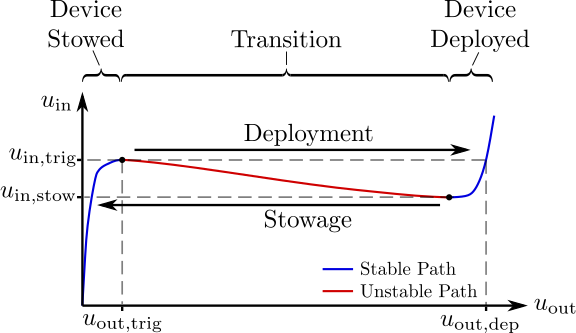
\includegraphics[width=0.5\textwidth]{IntroductionImages/Desired_Path_V4.png}
			\caption{\centering Ideal behaviour of the passively actuated spoiler concept. (Reprinted from \cite{Wheatcroft_2023})}
			\label{fig:DesiredPath}
		\end{figure}
       
	  \subsection{Research Objectives}
        The primary objective of the present work was to develop a method to experimentally demonstrate sequential instability to display the feasibility of the passively actuated spoiler concept proposed by Wheatcroft et al. in \cite{Wheatcroft_2023}. The secondary objective was to characterise the relationship between the response of the system and the properties of both the Euler strut and laminate. 
   
		
	\section{Manufacturing}
    \subsection{Laminate}
    \subsubsection{Cutting}
    To mitigate dust generation SE-84LV laminate was cut with a water-lubricated wet diamond tile cutter by RUBI. To mitigate the risk of chipping the thin ply was cut with stainless steel Glass Fibre Shears by Wilkinson.
    \subsection{Test Rig}
    \subsubsection{MDF Aerofoil}
    Limitation in the availability of workshops r(intrro). 
    \begin{figure}[h]
        \centering
        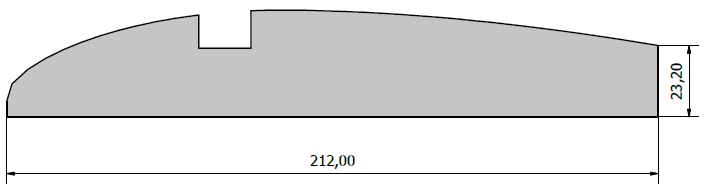
\includegraphics[width = 0.5\linewidth]{Figures/Jan/laser2.png}
        \caption{Caption}
        \label{fig:laser}
    \end{figure}
    Thirty sections illustrated in~\Cref{fig:laser} were cut out of \SI{10}{\milli \meter} thick MDF using Trotec SP 500. Sections were later glued using PVA-based glue. After curing for 24 hours the part  was sanded with an oscillatory sander (BRAND MISSING) using 80-grid sandpaper. Pilot holes for brass inserts were drilled out and the tool surface was painted black. Brass inserts (BRand missing) were placed in pre-drilled holes and were hammered down.
    \subsubsection{Boundary Conditions}
    \begin{figure}[h!]
        \centering
        %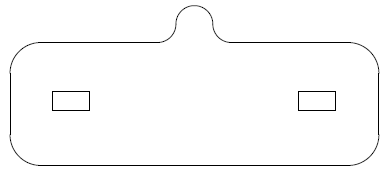
\includegraphics[width = \linewidth]{Figures/Jan/nipple.png}
        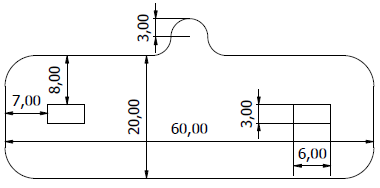
\includegraphics[width = \linewidth]{Figures/Jan/nippleNumber.PNG}
        \caption{Caption}
        \label{fig:nipple}
    \end{figure}
    \section{Numerical Modelling}
    ABAQUS was used for the finite element analysis of the strut-spoiler system. The Euler strut was modelled with beam elements and the spoiler used composite shell elements, as seen in \cref{fig:ModelAssem}. The spoiler was designed to follow the profile of the NACA 3412 aerofoil. 
    A tie constraint was applied at the centre of the strut and at the centre of the equivalent quarter-chord position of the spoiler (point A in \cref{fig:ModelAssem}). A mesh sensitivity study, outlined in \cref{fig:MeshSens} was also performed. Following from \cite{Wheatcroft_2023}, the spoiler is clamped at the leading edge and the nodes at point B are constrained to only move in the XZ plane. Additionally, the Euler Strut has clamped-clamped edge constraints. 

        \begin{figure}[!h]
        \footnotesize
        \centering
        \includesvg[width=0.5\textwidth]{ModellingImages/MeshSens.svg}
        \caption{ XX }
        \label{fig:MeshSens}
    \end{figure}
    \normalfont
    %\\
    The Euler strut was modelled as steel ($E$ = \SI{200}{GPa}, $\nu$ = \SI{0.3}{}) and the spoiler was modelled as one of two laminates.  The properties of the two laminates are shown in \cref{tab:ModelProp}.
    %\\
    
    In order to model the non-linear behaviour and to map the post-buckling response, a Riks step was used. A compressive displacement of \SI{1}{\milli\meter} was prescribed to both ends of the column in this step. The first buckling event is the Euler buckling of the Euler strut. At the point of buckling, the column reaches a pitchfork bifurcation. In order to bring the response down the desired equilibrium path (buckling in the positive $y$ direction, into the spoiler), an imperfection was seeded into the model. The imperfection took the form of a 2.5 N force acting in the positive $y$ direction at point A. This force was assigned to the model before the Riks step, to ensure the force stays constant during the analysis. Naturally, any imperfection would impact the response. For example, \cref{fig:Imperfect}, displays the difference in results when a \SI{5}{\newton} force is used instead of the \SI{2.5}{\newton} force. The tip displacement at zero axial beam displacement is higher for the former case. This results in a lower axial beam displacement for any given vertical trailing edge displacement, meaning that the spoiler would snap through at a lower applied displacement. The chosen \SI{2.5}{\newton} force seeds a \SI{0.10}{\milli\meter} vertical displacement to the centre of the beam, \SI{0.014}{\percent} of the total length of the beam. For the experimental beam, the imperfections would likely be larger than this and they are also likely to vary greatly. To simplify the comparison between the numerical and experimental results, a beam with minimal imperfections was modelled, so a nudge force of \SI{2.5}{\newton} was used. 

    \begin{figure}[!h]
        \footnotesize
        \centering
        \includesvg[width=0.5\textwidth]{ModellingImages/Imperfections.svg}
        \caption{ XX }
        \label{fig:Imperfect}
    \end{figure}
    \normalfont
   % \\

    The SE 84LV/ HEC laminate has extension-twist coupling. Therefore, the spoiler made from this laminate would experience thermal warping, when it cools after cure. This thermal warping was incorporated into the model for using the SE 84LV/ HEC laminate. Generic coefficients of thermal expansion (CTE) values were assigned to the laminate ($1\cdot10^{-6}K^{-1}$ and $3.5\cdot10^{-5}K^{-1}$, for the CTE parallel and perpendicular to the fibre direction, respectively). To minimise warping, a low temperature was chosen for the cure dwell time, of 80\;$^\circ C$. Therefore, a temperature field of -60\;$^\circ C$ was applied to the model to allow the analysis of the risk to be carried out on the warped laminate. However, the North Thinply 402/ T1000 laminate has no extension-twist coupling, so there was no temperature field applied in its analysis. 


    \begin{table*}[]
    \centering
    \small
     \caption{ Material properties of ... }
     \label{tab:ModelProp}
    \begin{tabular}{|l|l|l|l|l|l|l|l|l|}
    \hline
    \textbf{Laminate}   &  \textbf{Layup}   & $\mathbf{t}$ & $\mathbf{E_{11}}$ & $\mathbf{E_{22}}$ & $\mathbf{G_{12}}$ & $\mathbf{G_{13}}$ & $\mathbf{G_{23}}$ & $\mathbf{\nu_{12}}$ \\ 
    && \textbf{{[}mm{]}} & \textbf{{[}GPa{]}} & \textbf{{[}GPa{]}} & \textbf{{[}GPa{]}} & \textbf{{[}GPa{]}} & \textbf{{[}GPa{]}} &  \\ 
    \hline
    North Thinply  & [45/-45$_{2}$/45/0/-45/45$_{2}$/-45] & 0.032               & 145                   & 8.8                   & 4.5                    & 4.5                    & 4.5                    & 0.3          \\ 
     402/ T1000 &&                &                    &                   &                  &                    &                   &          \\ 
    \hline
    SE 84LV/ HEC            & [45/-45/0/45/-45] & 0.169               & 134                   & 8.3                   & 4                      & 4                      & 3.1                    & 0.314        \\ \hline
    \end{tabular}
    \end{table*}
    \normalfont


    \begin{figure*}[!h]
        \centering
        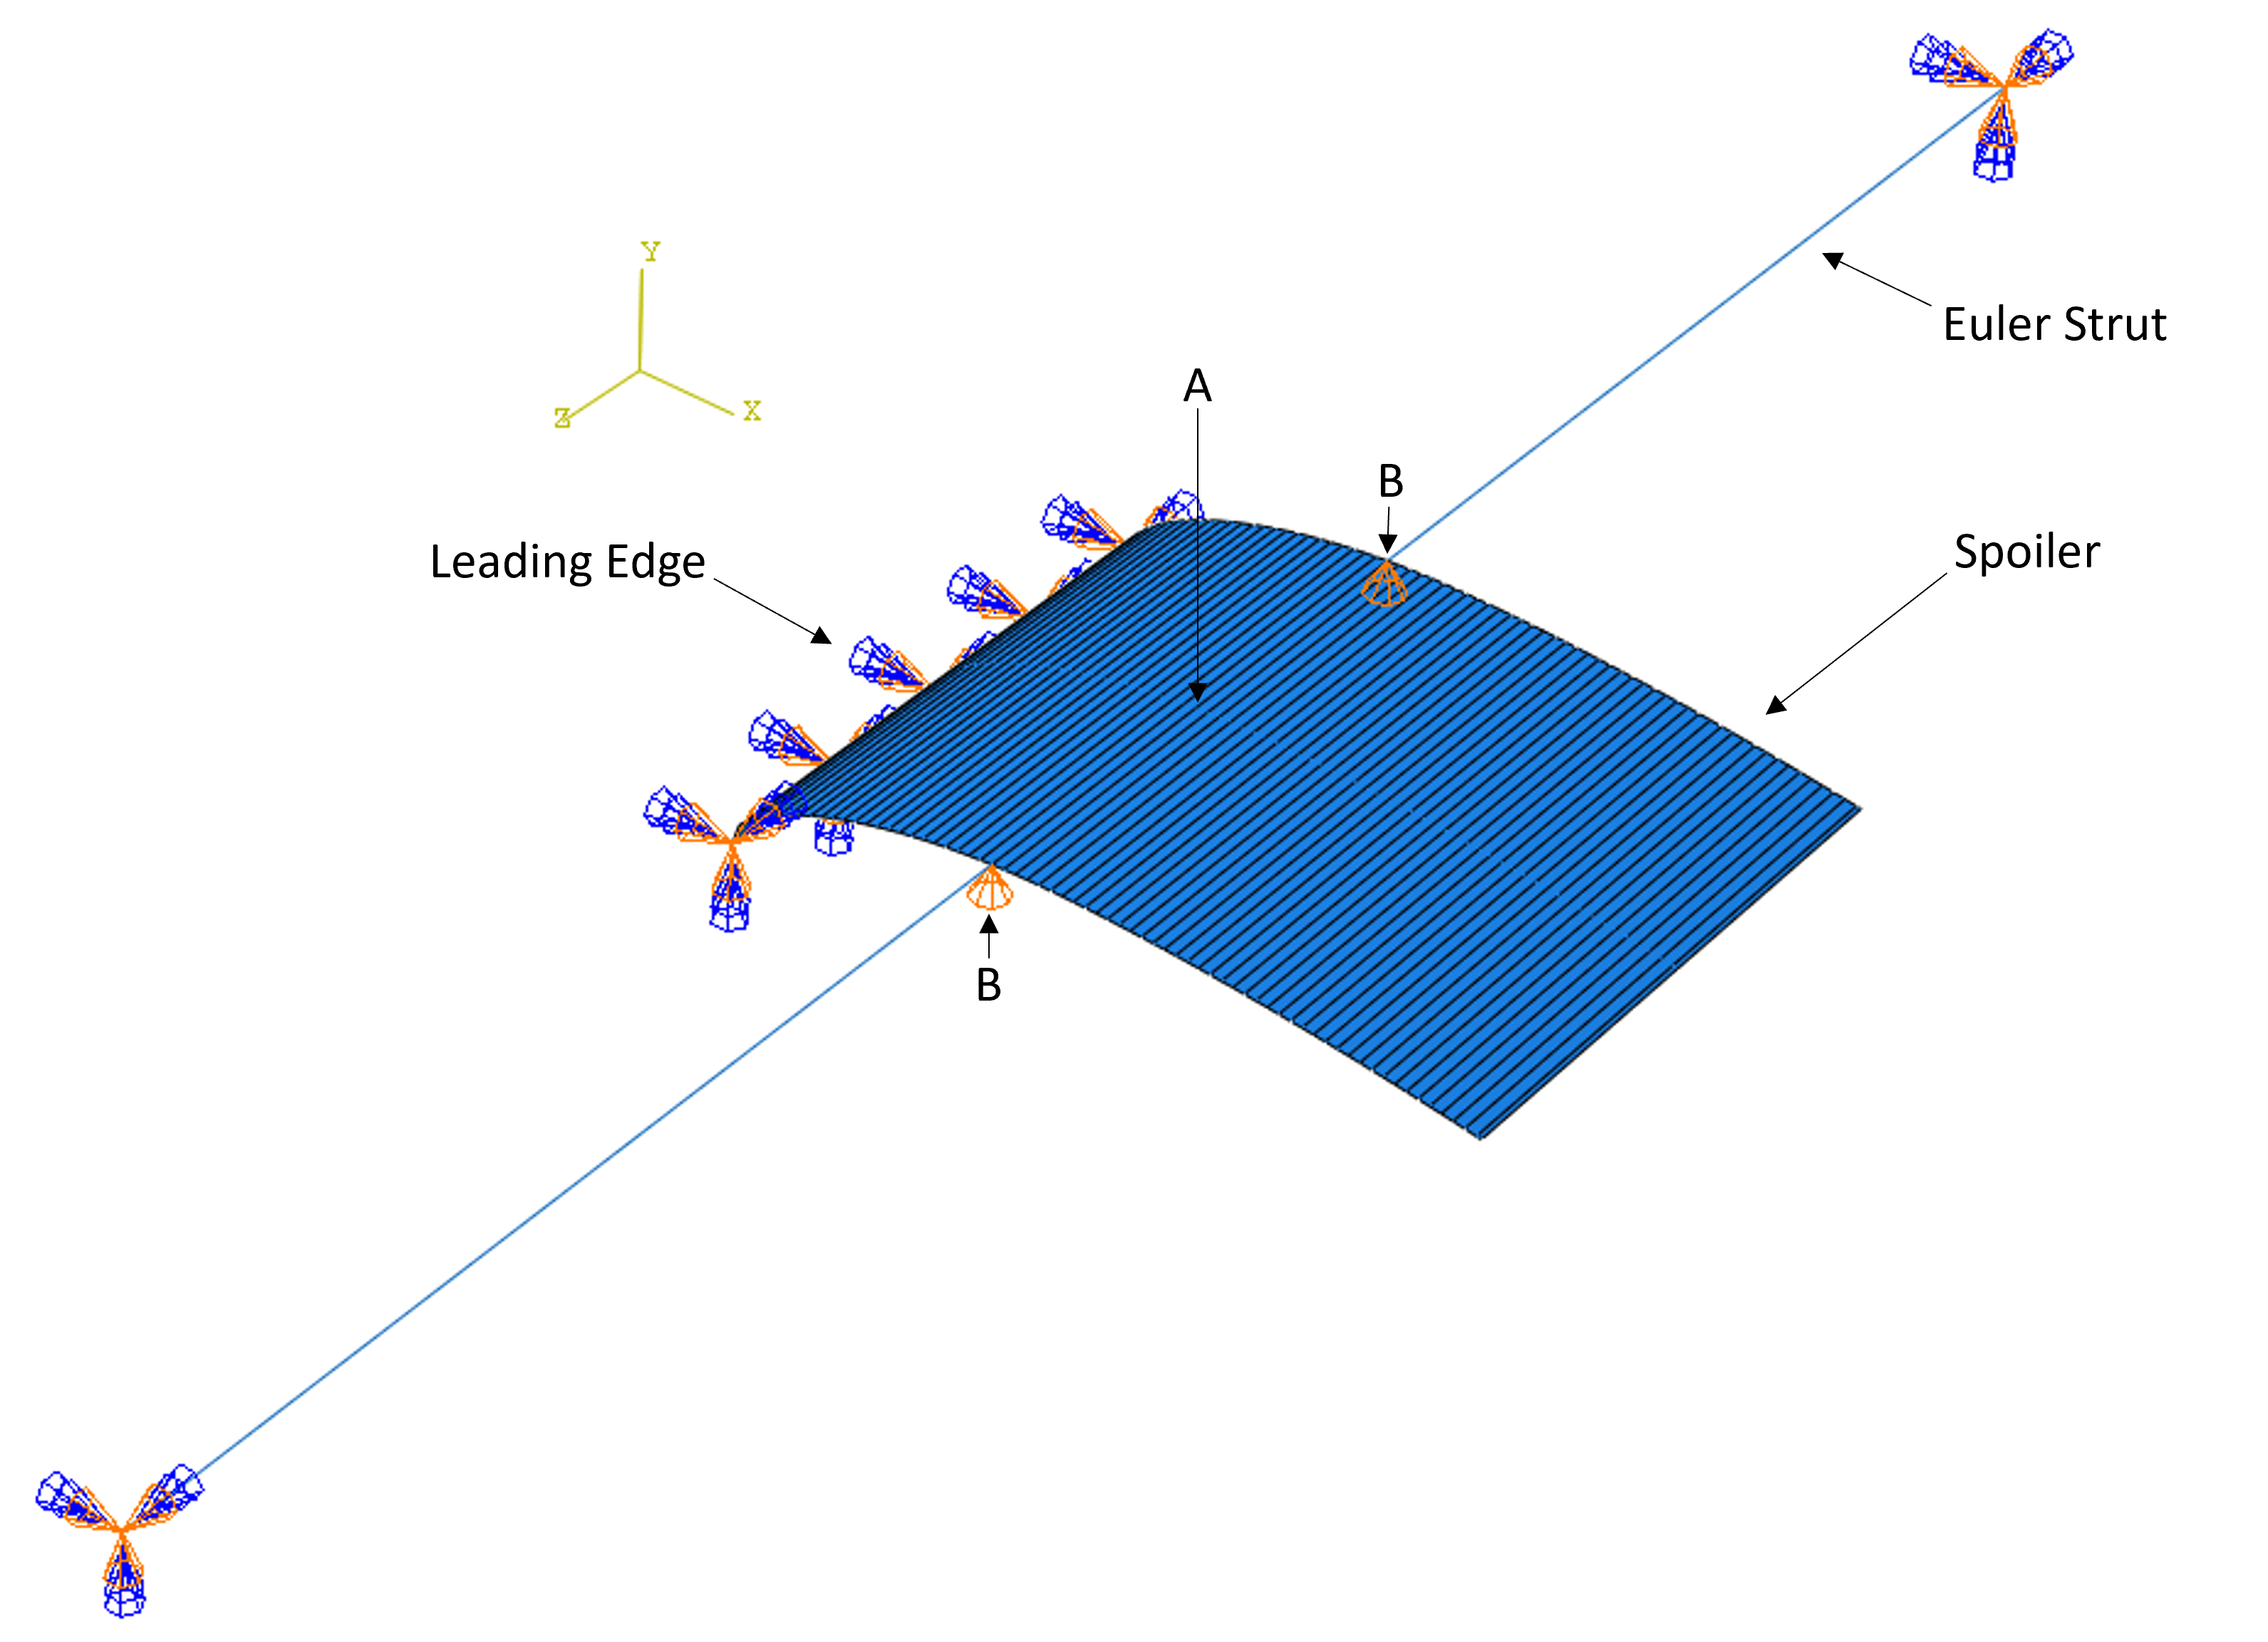
\includegraphics[width=\textwidth]{ModellingImages/ModelAssem.png}
        \caption{ XX }
        \label{fig:ModelAssem}
    \end{figure*}
	
    \section{Testing Procedure}

    \subsection{Requirements}
    % Asaad

    \subsection{Set Up}
    % Schimadzu - Asaad
    % Force Sensor - Asaad
    % Camera/DIC - Gokhan
    % Speckle/Calibration - Gokhan
	
	\section{Results}

    \subsection{Post Processing}

    %	Subset Optimisation – Jacopo/Gokhan
    %   Match ID vs DaVinci - Jacopo/Gokhan
    %   Beam vs Crosshead Displacement – Jacopo/Anna

    \subsection{Numerical Results}
    $u_{in}$ vs $u_{out}$ graphs which show the displacement response of the system are shown in 
	
    \subsection{Experimental Results}
    
    % Strain Maps – Jacopo/Anna/Asaad
    % Uin vs Uout – Jacopo/Anna/Asaad
    % Fin vs Fc – Jacopo/Anna/Asaad
    % Fc vs Uout,c – Jacopo/Anna/Asaad


	\section{Conclusion}

 -
	
	\newpage
    \printbibliography
	
\end{document}

%%TEMPLATES
%%PNG or JPEG files
\begin{figure}[!h]
	\centering
	\includegraphics[height=8cm]{}
	\caption{Caption}
	\label{fig:}
\end{figure}
%% SVG Files
\begin{figure}[!h]
	\centering
	\includesvg[height=8cm].svg}
	\caption{Caption}
	\label{fig:}
\end{figure}
	\subsection{Equations}
	Here is an example of an equation:
	\begin{equation}
		f(x) = x^2 + 2x + 1
	\end{equation}
	
	\subsection{Tables}
	Here is an example of a table:
	\begin{table}[htbp]
		\centering
		\caption{Example Table}
		\label{tab:example}
		\begin{tabular}{|c|c|c|}
			\hline
			\textbf{Column 1} & \textbf{Column 2} & \textbf{Column 3} \\
			\hline
			Row 1, Column 1 & Row 1, Column 2 & Row 1, Column 3 \\
			\hline
			Row 2, Column 1 & Row 2, Column 2 & Row 2, Column 3 \\
			\hline
			Row 3, Column 1 & Row 3, Column 2 & Row 3, Column 3 \\
			\hline
		\end{tabular}
	\end{table}
	
	\subsection{Figures}
	Here is an example of a figure:
	\begin{figure}[htbp]
		\centering
		\includegraphics[width=0.4\textwidth]{example-image-a}
		\caption{Example Figure}
		\label{fig:example}
	\end{figure}